\documentclass[aps,prb,superscriptaddress,showpacs,reprint,lengthcheck]{revtex4-1}
%%%%%%%%%%%%%%%%%%%%%%%%%%%%%%%%%%%%%%%%%%%%%%%%%%%%%%%%%%%%%%%%%%%%%%%%%%%%%%%%%%%%%%%%%%%%%%%%%%%%%%%%%%%%%%%%%%%%%%%%%%%%%%%%%%%%%%%%%%%%%%%%%%%%%%%%%%%%%%%%%%%%%%%%%%%%%%%%%%%%%%%%%%%%%%%%%%%%%%%%%%%%%%%%%%%%%%%%%%%%%%%%%%%%%%%%%%%%%%%%%%%%%%%%%%%%
\usepackage{amsmath}
\usepackage{graphicx}
\usepackage{subfig}

\setcounter{MaxMatrixCols}{10}


\newcommand{\vk}{\ensuremath{\mathbf{k}}}
\providecommand{\vr}{\ensuremath{\mathbf{r}}}
\newcommand{\gk}{\ensuremath{{g}(\mathbf{k})}}
\newcommand{\vp}{\ensuremath{\mathbf{p}}}
\newcommand{\gp}{\ensuremath{{g}(\mathbf{p})}}
\newcommand{\vq}{\ensuremath{\mathbf{q}}}
\newcommand{\Fo}{\ensuremath{\mathbf{F_0}}}
\newcommand{\E}{\ensuremath{\mathbf{E}}}
\newcommand{\A}{\ensuremath{\mathbf{A}}}
\newcommand{\J}{\ensuremath{\mathcal{J}}}
\newcommand{\ket}[1]{\ensuremath{\left|#1\right>}}
\newcommand{\bra}[1]{\ensuremath{\left<#1\right|}}
\newcommand{\twoe}{\ensuremath{2\epsilon_\vk-\E_1}}
\newcommand{\nth}[1]{\ensuremath{\frac{1}{#1}}}
\newcommand{\br}[1]{\ensuremath{\left(#1\right)}}
\newcommand{\mbr}[1]{\ensuremath{\left[#1\right]}}
\newcommand{\bbr}[1]{\ensuremath{\left\{#1\right\}}}
\newcommand{\av}[1]{\ensuremath{\bigl<{#1}\bigr>}}
\newcommand{\avv}[2][\nu]{\av{#1{\lvert{#2}\rvert}#1}}
\newcommand{\avt}[2]{\av{{#1}|{#2}}}
\newcommand{\avtu}[1]{\av{T_\tau#1}}
\newcommand{\zmatrix}{\ensuremath{\br{\begin{smallmatrix}0&0\\0&0\end{smallmatrix}}}}
\newcommand{\fmtrx}[4]{\ensuremath{\br{\begin{smallmatrix}#1&#2\\#3&#4\end{smallmatrix}}}}
\newcommand{\smtrx}[6]{\ensuremath{\br{\begin{smallmatrix}#1&#2\\#3&#4\\#5&#6\end{smallmatrix}}}}
\newcommand{\vz}{\ensuremath{v^{\beta\alpha}_{\vk,\vk}}}
\providecommand{\abs}[1]{\ensuremath{\lvert{#1}\rvert}}
\newcommand{\com}[2]{\ensuremath{\mbr{#1,#2}}}
\newcommand{\D}{\ensuremath{\mathit{D}}}
\providecommand{\hm}{\ensuremath{\frac{\hbar^2}}{2m}}
\providecommand{\pdiff}[2]{\ensuremath{\frac{\partial{#1}}{\partial{#2}}}}
\providecommand{\dpdiff}[2]{\ensuremath{\frac{\partial^2{#1}}{\partial{{#2}^2}}}}
\providecommand{\H}{\ensuremath{\mathcal{H}}}
\providecommand{\wt}[1]{\widetilde{#1}}
\newcommand{\efo}{\epsilon_{F_0}}
\newcommand{\fo}{\ensuremath{\ket{F_0}}}
\renewcommand{\E}{\ensuremath{\mathcal{E}}}


\begin{document}

\title{Coboson Derivation of Richardson's Equations for Cooper pairs}
\author{Monique Combescot}
\affiliation{Institut des NanoSciences de Paris, Universite Pierre et Marie Curie, CNRS, Campus Boucicaut, 140 rue de Lourmel, 75015 Paris, France}
\affiliation{Department of Physics, University of Illinois at Urbana-Champaign, 1110 W Green St, Urbana, IL, 61801}
\author{Guojun Zhu}
\affiliation{Department of Physics, University of Illinois at Urbana-Champaign, 1110 W Green St, Urbana, IL, 61801}

\date{\today}

\begin{abstract}
Five years after the milestone paper by Bardeen, Cooper, Schrieffer (BCS) in which
superconductivity is tackled within the grand canonical ensemble, 
Richardson found a smart way to approach the problem within the canonical ensemble: He succeeded to
write down the \textit{exact analytical form} of the Schr\"{o}dinger equation eigenstate for
an arbitrary number of Cooper pairs interacting through the standard BCS
potential. We here rederive his result using a commutation technique similar to the one we
have recently developed for many-body effects between composite bosons
(cobosons in short). This derivation makes crystal clear the physical origin of the various terms, in particular the fact that difference
between a collection of single Cooper pairs and the BCS condensate are solely due to the Pauli exclusion principle
through electron exchanges between pairs. Our procedure gives also hints on
why, as we very recently found, the interaction part of the $N$-pair ground state energy
increases with pair number as $N(N-1)$ only from the dilute to the dense regime
of pairs. Finally, in this work, we briefly question the validity of the BCS wave
function ansatz in the light of Richardson's exact solution.
\end{abstract}

\pacs{74.20.Fg, 03.75.Hh, 67.85.Jk}
\maketitle


It is known for quite a long time that the Pauli exclusion principle
plays a key role in superconductivity. None the less, the
precise way Pauli blocking transforms a collection of single Cooper pairs into a BCS
condensate, has been understood quite recently only. This precise understanding goes through
the study of Cooper pairs not within the grand canonical ensemble as done in the
standard BCS theory, but within the canonical ensemble. It is however  known that to handle the
Pauli exclusion principle between a fixed number of interacting fermions is quite difficult, especially when these fermions are paired. 
Turning to the grand canonical ensemble makes the task far easier. Yet, adding fermion pairs one by
one is the best way to precisely follow the increasing effect of Pauli
blocking from the dilute to the dense regime of pairs.

Five years after the milestone paper on superconductivity by Bardeen,
Cooper, Schrieffer\cite{BCS}, Richardson succeeded to solve this N-body problem exactly and to formally write
the exact form of the Schr\"{o}dinger equation eigenstates for an arbitrary number $N$ of Cooper pairs%
\cite{Richardson1,Richardson2}. This exact solution is expressed in terms
of $N$ parameters, $R_{1}$,... $R_{N}$ which are shown to be solutions of $N$ coupled
non-linear equations, the energy of these $N$ pairs reading as $E
_{N}=R_{1}+...+R_{N}$. Although this exact form is definitely quite smart, to
use it in practice is not that easy: Except in the infinite $N$ limit for which the BCS energy can be recovered \cite{Richardson3}, these equations for $R_{1}$,... $R_{N}$  did not have, up to now, analytical solution for arbitrary $N$ and arbitrary interaction strength, so that they were approached through
numerical procedures\cite{Duk,delft} only. This is probably why the Richardson's equations have not had so far the
attention they deserve among the superconductor community. Nowadays, these equations 
are commonly addressed numerically to study superconducting granules with a small number of pairs\cite{Duk}.

Last year, we reconsidered these Richarson's equations because we wanted to reveal the deep connection which exists between two well-known problems, namely the
one-pair problem solved by Cooper and the many-pair problem considered by Bardeen, Cooper and Schrieffer. 
These two problems have intrinsic similarities: In
both cases, there is a ``frozen'' core of non-interacting electrons. Above this core, there is
a potential layer with attraction between up and
down spin electrons. In the one-pair problem, this layer contains one electron pair 
only, while in the standard BCS configuration, the
layer is half-filled - the potential layer being said to extend symmetrically 
on both sides of the Fermi level which is just equivalent to half filling.
It is clear that, by adding more and more pairs into the potential layer, we can 
continuously go from the one-pair problem studied by Cooper to the dense regime studied by Bardeen, Cooper and Schrieffer. 

Although, at the present time, such a continuous pair increase
does not seem easy to achieve experimentally, this increase can at least be seen as a 
gedanken experiment to study the evolution of the energy spectrum when
the filling of the potential layer is changed, in order to understand the exact role of the Pauli
exclusion principle in superconductivity. 
This procedure can also be
seen as a simple but well-defined toy model to tackle the BEC-BCS crossover
since, by changing the number of pairs, we change their overlap. 
Such an overlap change has already been considered by Eagles \cite{Eagle}, 
and also by Leggett \cite{LeggettCrossover}, but through the change of the interaction strength between pairs. The number of pairs being then fixed, Pauli blocking does not change in this overlap change while it does when we increase the pair number, so that the two kinds of overlap change are not totally equivalent.

Since the Richardson's procedure allows one to fix the pair number and vary 
this number at will from one to half filling, we seriously reconsidered 
solving these equations analytically in order to evidence the effect of Pauli blocking. By turning to their dimensionless form, we succeeded to
find an analytical way to solve these equations in the dilute regime of
pairs \cite{paper1}. Indeed, these equations do have a small dimensionless parameter, namely $1/{%
N_{c}}$ where $N_{c}$ is the number of pairs from which overlap between single pairs would start. 
This allowed us to demonstrate in the dilute limit on
the single Cooper pair scale, i.e., for $N$ arbitrary large but $N/N_{c}$ small, that the energy of $%
N$ Cooper pairs reads in the large sample limit as 
\begin{equation}
E_{N}=N\left[ \left( 2\epsilon _{F_{0}}+\frac{N-1}{\rho _{0}}%
\right)-\epsilon _{c}\left( 1-\frac{N-1}{N_{\Omega }}\right) \right]
\label{eq:eN}
\end{equation}%
$\epsilon _{F_{0}}$ is the Fermi level energy of the frozen sea.  $\rho
_{0} $ is the density of states within the potential
layer, taken as constant. $N_{\Omega }=\rho _{0}\Omega $ is the number of free pair states in this
layer, $\Omega $ being the potential layer extension. $\epsilon _{c}\approx
2\Omega \exp \left( -2/\rho _{0}V\right) $ is the single pair binding
energy for a small potential amplitude $V$ (weak-coupling limit).

Although our actual derivation imposes $N/N_{c}$ small, it turns out that this result is also valid in the dense BCS regime,
where pairs strongly overlap. Indeed, the first term of Eq.\eqref{eq:eN} is
the exact energy of $N$ pairs in the normal state since it is nothing but 
\begin{multline}
{E}_{N}^{\text{(}normal)}= \\
2\left[\epsilon _{F_{0}}+\left( \epsilon _{F_{0}}+1/\rho _{0}\right) +\cdots
\;+\left( \epsilon _{F_{0}}+(N-1)/\rho _{0}\right)\right]
\end{multline}%

For a number of pairs corresponding to fill half the potential layer, which precisely is 
the BCS configuration, Eq.\eqref{eq:eN} gives a condensation
energy equal to 
\begin{equation}
{E}_{N}^{\text{(}normal)}-{E}_{N}=\frac{N_{\Omega }}{2}\frac{%
\epsilon _{c}}{2}=\frac{1}{2}\rho _{0}\Omega ^{2}e^{-2/\rho _{0}V}
\end{equation}%
This result exactly matches the one derived by Bardeen, Cooper, Schrieffer within the grand canonical
ensemble using the BCS wave function ansatz, namely $\rho _{0}\Delta ^{2}/2$ since the gap $\Delta $ reads as $%
2\omega _{c}\exp \left( -1/\rho _{0}V\right) $ where $2\omega _{c}$ is nothing but the
potential layer extension $\Omega $. It also is remarkable to 
note that if we extend the BCS grand canonical derivation originally performed for half filling, to
non-symmetrical configurations, Eq.\eqref{eq:eN} remains valid.

The canonical approach we have used to reach Eq.\eqref{eq:eN}, based on solving 
Richardson's equations analytically, has the great advantage to follow the evolution of the
ground state energy when adding pairs one by one. This leads us to, in a natural way, 
associate the second term in the RHS of Eq.%
\eqref{eq:eN}, namely $\epsilon _{c}\left[ 1-\left( N-1\right) /N_{\Omega }%
\right] $, with the average ``pair binding energy'' in the $N$-pair configuration: for $N=1$, this quantity exactly matches the
single-pair binding energy found by Cooper, while in the dense regime, it 
gives the condensation energy per pair. This is of importance for physical understanding because this pair energy
allows us to connect the dilute and dense regimes of pairs within the same framework.

We see that the pair binding energy, as defined
above, decreases when $N$ increases. This decrease is entirely due to
Pauli blocking, the number of  states in
the potential layer, available to form correlated pairs, decreasing when $N$ increases. 
A pictorial way to
understand the binding energy decrease when $N$ increases is through the
so-called ``moth-eaten'' effect: when pairs are added to the frozen Fermi sea $\left\vert
F_{0}\right\rangle $, they ``eat'' one by one, like little moths, the
states in the potential layer available to form  bound state. As
a result of this available state decrease, the bound state energy can only
decrease. 

Note that this pair binding energy decrease is at odd from
the common belief that in the dense BCS configuration, the Cooper pair
binding energy is of the order of the excitation gap since  $\Delta $ is far larger
than $\epsilon _{c}$. This common belief is obtained by splitting the
condensation energy $\rho _{0}\Delta ^{2}/2$ as $(\rho _{0}\Delta )\Delta $
within an ``irrelevant'' $1/2$ prefactor. This procedure deliberately assigns to each pair an
energy equal to the gap, the number of pairs to fit the condensation energy
then being $\rho _{0}\Delta $, i.e., the number of pairs in a gap layer. These $\rho
_{0}\Delta $ pairs have been called ``virtual pairs'' by Schrieffer.
Their number is definitly far smaller than the number of pairs $N_{\Omega }/2$ feeling
the potential. As a direct consequence, their energy is far larger than the average binding energy $%
\epsilon _{c}/2$ of the pairs which feel the potential. These virtual pairs in fact correspond
to excitations across the Fermi sea $\left\vert F\right\rangle $ made of $%
N+N_{0}$ \textit{noninteracting} pairs, $N_{0}$ being the number of pairs in
the frozen core $\left\vert F_{0}\right\rangle $. It is of importance to note that the concept of virtual
pairs is physically relevant in the dense regime only; in the
dilute regime, the Fermi level for noninteracting electrons is completely
washed out, all the pairs feeling the potential being essentially excited above this level.
Another unpleasant aspect of this virtual pair concept is that it tends to 
mask the obvious link which exists between the dilute and dense regimes of pairs. 
This probably is one of the reasons for Schrieffer's statement that the
isolated pair picture has little meaning in the dense regime
\cite{Schrieffer}. This statement was already questioned by Leggett who
showed that, in many respects, pairs in the dense limit are very similar to giant molecules made of two opposite spin electrons \cite{LeggettCrossover}. The result of Eq.(1) confirms Leggett's understanding. 

Since the key role of Pauli blocking in superconductivity is enlightened by
the expression of the $N$-pair energy reported in Eq.\eqref{eq:eN}, through the ``moth-eaten effect'' it contains, 
while this expression has been obtained by solving the
Richardson's equations analytically, it can be of interest to trace back the parts in
these equations which directly come from the Pauli exclusion principle.

In our recent works on the many-body physics of composite bosons - mostly concentrated on semiconductor excitons - we have
proposed a ``commutation technique'' which allows us to evidence the effects
of Pauli blocking between the fermionic components of these composite
bosons (cobosons in short). They appear through ``Pauli scatterings'' which describe fermion
exchanges in the absence of fermion interaction. These dimensionless
scatterings, when mixed with energy-like scatterings coming from interactions
between the coboson fermionic components, allow us to deal with fermion exchanges
between any number of composite particles in an exact way. For a review on
this formalism and its applications to the many-body physics of
semiconductor excitons, see Refs. \cite%
{CobosonPhysicsReports}.

In the present paper, we first develop such a commutation technique for up and down spin
electron pairs with zero total momentum, these being the elementary composite bosons on which Cooper pairs are constructed. We then use this commutation technique to derive in a quite
compact way, the form of the exact eigenstate for $N$ pairs interacting
through the reduced potential used by Bardeen, Cooper and Schrieffer. The Richardson's equations readily follow
from this approach. Its main advantage is to possibly trace back the physical origin of the terms in $1/(R_i-R_j)$. These differences actually come
from Pauli scatterings for fermion exchanges 
between up and down spin electron pairs. This understanding leads us to conclude that 
the Richardson's energies $R_i$  have $N$ different values just because 
of Pauli blocking between the Cooper pair components.

The paper is organized as follow:

In section \ref{sec:beta}, we present the commutation technique  appropriate to many-body effects between the free
electron pairs on which Cooper pairs are constructed. We derive their associated Pauli and interaction scatterings.

In section \ref{sec:rich}, we use this formalism to recover the Richardson's form of the
exact eigenstates for $N=1,2,3,\cdots$ pairs interacting through the reduced
BCS potential, in order to see how the solution for general $N$ develops. We
then analyze the precise role of Pauli blocking in this solution.

In section \ref{sec:conn}, we briefly question the BCS wave function ansatz for condensed pairs in the light of the exact form provided by the Richardson's procedure.

\section{Commutation Technique for free fermion pairs making Cooper pairs\label{sec:beta}}

\subsection{Exchange scattering}

We consider cobosons made of free fermion pairs having zero total
momentum. 
\begin{equation}
\beta^{\dagger}_\vk=a^{\dagger}_{\mathbf{k} }b^{\dagger}_{-\mathbf{k} }
\end{equation}
These pairs have one degree of freedom
only, namely $\mathbf{k}$. This has to be  contrasted to the
most general fermion pairs $a^{\dagger}_{\mathbf{k} _1}b^{\dagger}_{\mathbf{k%
} _2}$, such as Wannier exciton pairs, which have two, but has close similarity with Frenkel exciton pairs \cite{frenkel}, the index $\mathbf{k}$ being replaced by the excited ion sites. In the case of Cooper pairs, $a^{\dagger}_{\mathbf{k} }$ creates a spin up electron with momentum $\mathbf{k}$ while $b^{\dagger}_{\mathbf{-k} }$ creates a down spin electron with momentum $\mathbf{-k}$. 

It is straightforward to show that the creation operators of the free fermion pairs commute 
\begin{equation}  \label{eq:bCom}
\left[\beta^{\dagger}_{\mathbf{k} ^{\prime}},\beta^{\dagger}_{\mathbf{k} }%
\right]  =0
\end{equation}
So that the pairs are bosons (????)  particles.  It is however worth noting that while ${(a^{\dagger}_{\mathbf{k}})} ^2=0$
simply follows from the anticommutation of $a^{\dagger}_{\mathbf{k} }$
operators, the cancellation of ${(\beta^{\dagger}_{\mathbf{k}})} ^2$ does not follow from Eq.\eqref{eq:bCom}, but from the fact that ${(\beta^{\dagger}_{\mathbf{k}})} ^2$  contains ${(a^{\dagger}_{\mathbf{k}})} ^2$. The ${(\beta^{\dagger}_{\mathbf{k}})} ^2$  cancellation which comes from Pauli blocking, can seem to be lost
when working with pair operators instead of  single fermion operators to pair operators. We will see that this Pauli blocking is yet preserved in the commutation algebra for
free fermion pairs we are going to develop.

If we now turn to creation and annihilation operators, their commutator reads
\begin{equation}  \label{eq:betacom}
\left[\beta_{\mathbf{k} ^{\prime}},\beta^{\dagger}_{\mathbf{k} }\right] 
=\delta_{\mathbf{k} ^{\prime}\mathbf{k} }-\mathit{D} _{\mathbf{k} ^{\prime}%
\mathbf{k} }
\end{equation}
where the deviation-from-boson operator of two zero-momentum free fermion $\mathit{D} _{\mathbf{k} ^{\prime}\mathbf{k%
} }$ reduces to 
\begin{equation}  \label{eq:D}
\mathit{D} _{\mathbf{k} ^{\prime}\mathbf{k} }=\delta_{\mathbf{k} ^{\prime}%
\mathbf{k} }\left(a^{\dagger}_{\mathbf{k}}a^{}_{\mathbf{k}
}+b^{\dagger}_{-\mathbf{k} }b^{}_{-\mathbf{k}
}\right) 
\end{equation}
This operator which would be  zero for fermion pairs  taken as
elementary bosons, allows us to generate the Pauli scatterings for fermion
exchanges between composite bosons in the absence of fermion interaction. Following our work on excitons\cite%
{CobosonPhysicsReports}, these are formally defined through 
\begin{equation}
\left[\mathit{D} _{\mathbf{k} ^{\prime}_1\mathbf{k} ^{}_1},\beta^{\dagger}_{%
\mathbf{k} _2}\right]  =\sum_{\mathbf{k} ^{\prime}_2}\left\{\lambda\left(%
\begin{smallmatrix}\vk'_2&\vk_2\\\vk'_1&\vk_1\end{smallmatrix}\right) 
+\left(\mathbf{k} ^{\prime}_1\leftrightarrow\mathbf{k} ^{\prime}_2\right)
\right\} \beta^{\dagger}_{\mathbf{k} ^{\prime}_2}
\end{equation}
By noting that

\begin{equation}  \label{eq:aBeta}
\left[a^{\dagger}_{\mathbf{k} }a^{}_{\mathbf{k} },\beta^{\dagger}_{\mathbf{p}
}\right]  =\delta_{\mathbf{k} \mathbf{p} }\beta^{\dagger}_{\mathbf{p} }=%
\left[b^{\dagger}_{-\mathbf{k} }b^{}_{-\mathbf{k} },\beta^{\dagger}_{\mathbf{%
p} }\right]  
\end{equation}
it is then easy to show that 
\begin{equation}  \label{eq:Dcom}
\left[\mathit{D} _{\mathbf{k} ^{\prime}_1\mathbf{k} ^{}_1},\beta^{\dagger}_{%
\mathbf{k} _2}\right]  =2\beta^{\dagger}_{\mathbf{k} ^{}_2}\delta_{\mathbf{k} _1%
\mathbf{k} _2}\delta_{\mathbf{k} ^{\prime}_1,\mathbf{k} ^{}_2}
\end{equation}
This leads us to identify the Pauli scattering of two zero momentum free fermion pairs which appears in Eq.(8) with a
product of Kronecker symbols 
\begin{equation}  \label{eq:pauliscattering}
\lambda\left(\begin{smallmatrix}\vk'_2&\vk_2\\\vk'_1&\vk_1\end{smallmatrix}%
\right)  =\delta_{\mathbf{k} ^{\prime}_1\mathbf{k} ^{}_1}\delta_{\mathbf{k}
^{\prime}_2\mathbf{k} ^{}_2}\delta_{\mathbf{k} ^{}_1\mathbf{k} ^{}_2}
\end{equation}
Such a simple expression results from the fact that fermions are free, ???? also because they have one degree of freedom only.
Actually, this Pauli scattering is just the one we expect for fermion exchanges between $\left(\mathbf{k} _1,\mathbf{k} _2\right) $ pairs in the abscence of fermion interaction,
as visualized by the diagram of Fig.(1a). Indeed, from this
diagram, it is clear that we must have $\left(\mathbf{k} ^{\prime}_1=\mathbf{%
k} ^{}_1,\mathbf{k} ^{\prime}_2=\mathbf{k} ^{}_2\right) $ and $\left(-\mathbf{k}
^{\prime}_2=-\mathbf{k} ^{}_1,-\mathbf{k} ^{\prime}_1=-\mathbf{k} ^{}_2\right) $:
this just gives $\delta_{\mathbf{k} ^{\prime}_1\mathbf{k} ^{}_1}\delta_{\mathbf{%
k} ^{\prime}_2\mathbf{k} ^{}_2}\delta_{\mathbf{k} ^{}_1\mathbf{k} _2}$ in
agreement with Eq.\eqref{eq:pauliscattering}.

\begin{figure}[htb]
\centering
\par
  \subfloat[][]{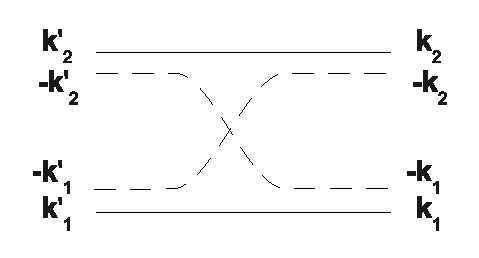
\includegraphics[width=0.3\textwidth]{lambda1.eps}\label{fig:lambda}}\qquad
 \subfloat[][]{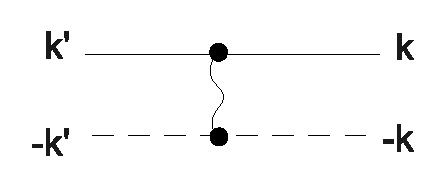
\includegraphics[width=0.3\textwidth]{direct1.eps}\label{fig:direct}}\\
  \subfloat[][]{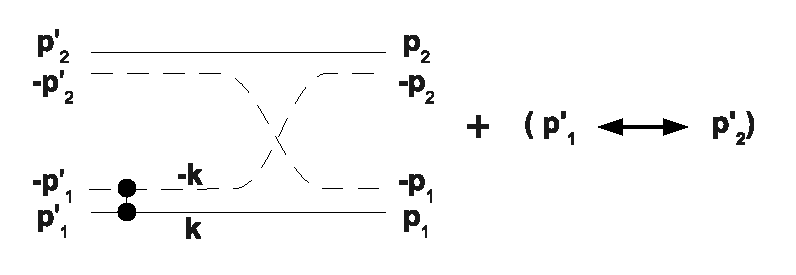
\includegraphics[width=0.4\textwidth]{chi1.eps}\label{fig:chi}} 
\par
\caption{Shiva diagram of free pairs }
\normalsize
\begin{flushleft}	
\subref{fig:lambda} Pauli scattering $\lambda\left(%
\begin{smallmatrix}\vk'_2&\vk_2\\\vk'_1&\vk_1\end{smallmatrix}\right)  $ for
electron exchange between two free pairs $\left(\mathbf{k} _1,\mathbf{k}
_2\right) $, as given by Eq.\eqref{eq:pauliscattering}. Up spin electrons
are represented by solid lines, down spin electrons by dashed lines. 
\par\subref{fig:direct} The BCS potential given in Eq.\eqref{eq:vbcs}
transforms a $\mathbf{k} $ pair into a $\mathbf{k} ^{\prime}$ pair, with a
constant scattering $-V$, in the case of a separable potential $v_{\mathbf{k}
^{\prime}\mathbf{k} }=-V\,w_{\mathbf{k} ^{\prime}}w_{\mathbf{k} }$.
\par
\subref{fig:chi} Interaction scattering $\chi\left(%
\begin{smallmatrix}\vp'_2&\vp_2\\\vp'_1&\vp_1\end{smallmatrix}\right)  $
between two free pairs, as given in Eq.\eqref{eq:interactSc}. Since the BCS
potential acts within one pair only, scattering between two pairs can
only come from exchange induced by the Pauli exclusion principle. 
\end{flushleft}

\end{figure}

\subsection{Interaction scattering}

To get the interaction scatterings associated to fermion interaction, we
first note that, for a free fermion hamiltonian 
\begin{equation}  \label{eq:h0}
H_0=\sum{\epsilon_\vk\left(a^{\dagger}_{\mathbf{k} } a^{}_{\mathbf{k}
}+b^{\dagger}_{\mathbf{k} } b^{}_{\mathbf{k} }\right) }
\end{equation}
Eq.\eqref{eq:aBeta} readily gives 
\begin{equation}  \label{eq:betaH}
\left[H_0,\beta^{\dagger}_\vp\right]  =2\epsilon_\vp\beta^{\dagger}_\vp
\end{equation}

In  standard BCS superconductivity, these fermion pairs interact through the reduced potential
\begin{equation}  \label{eq:vbcs}
V_{BCS}=\sum{v_{\mathbf{k} ^{\prime}\mathbf{k} }\beta^{\dagger}_{\mathbf{k}
^{\prime}}\beta^{}_{\mathbf{k} }}
\end{equation}
It is of importance to note that this potential fundamentally is a (1x1) potential in the fermion pair subspace since fermion $\mathbf{k}$ 
interacts with one fermion only of the other
species, namely fermion $\left(-\mathbf{k} \right)$(See Fig.(1b)). As a crucial consequence, this prevents direct interaction between two zero momentum pairs, the only way these pairs feel each other, i.e., interact in the most general sense, being from Pauli exclusion principle. 


  For this (1x1)
potential, we do have 
\begin{equation}  \label{eq:vbeta}
\left[V_{BCS},\beta^{\dagger}_\vp\right] 
=\gamma^{\dagger}_\vp+V^{\dagger}_\vp
\end{equation}
in which we have set $\gamma^{\dagger}_\vp=\sum_\vk\beta^{\dagger}_\vk{}v_{%
\mathbf{k} \mathbf{p} }$. The ``creation potential'' $V^{\dagger}_\vp$ of the free fermion pair 
$\mathbf{p} $ is given by 
\begin{equation}  \label{eq:betaV}
V^{\dagger}_\vp=-{\gamma^{\dagger}_\vp}\left(a^{\dagger}_{\mathbf{p} }a^{}_{%
\mathbf{p} }+b^{\dagger}_{-\mathbf{p} }b^{}_{-\mathbf{p} }\right) 
\end{equation}

While the $\gamma^{\dagger}_\vp$ part of Eq.\eqref{eq:vbeta} 
commutes with $%
\beta^{\dagger}_{\vp ^\prime}$, 
this is not so for the creation potential $%
V^{\dagger}_\vp$. Using Eq. (\ref{eq:aBeta}), its commutator precisely reads 
\begin{equation}\begin{split}  \label{eq:vpotbeta}
\left[V^{\dagger}_{\mathbf{p} _1},\beta^{\dagger}_{\mathbf{p} _2}\right] 
&=-2\delta_{\mathbf{p} _1\mathbf{p} _2}\gamma^{\dagger}_{\mathbf{p}
_1}\beta^{\dagger}_{\mathbf{p} _1}\\
&=-2\delta_{\mathbf{p} _1\mathbf{p} _2}\sum_\mathbf{k}\beta^{\dagger}_{\mathbf{k}}\beta^{\dagger}_{\mathbf{p} _1}v_{\mathbf{k}\mathbf{p} _1}
\end{split}\end{equation}
This allows us to identify the interaction scattering for free pairs with zero momentum,
formally defined as \cite{CobosonPhysicsReports}
\begin{equation}  \label{eq:vBeta}
\left[V^{\dagger}_{\mathbf{p} _1},\beta^{\dagger}_{\mathbf{p} _2}\right] 
=\sum\chi\left(\begin{smallmatrix}\vp'_2&\vp_2\\\vp'_1&\vp_1\end{smallmatrix}%
\right)  \beta^{\dagger}_{\mathbf{p} ^{\prime}_1}\beta^{\dagger}_{\mathbf{p}
^{\prime}_2}
\end{equation}
with a sequence of one (2x2) fermion exchange between two pairs and one (1x1) fermion interaction inside one pair. Indeed, this sequence leads to
\begin{equation}  \label{eq:interactSc}
\begin{split}
\chi\left(\begin{smallmatrix}\vp'_2&\vp_2\\\vp'_1&\vp_1\end{smallmatrix}%
\right)  &=-\sum_\vk\left\{v_{\mathbf{p} ^{\prime}_1\mathbf{k} }\lambda\left(%
\begin{smallmatrix}\vp'_2&\vp_2\\\vk&\vp_1\end{smallmatrix}\right)  +\left(%
\mathbf{p} ^{\prime}_1\leftrightarrow\mathbf{p} ^{\prime}_2\right) \right\} 
\\
&=-\left(v_{\mathbf{p} ^{\prime}_1,\mathbf{p} _1}\delta_{\mathbf{p}
^{\prime}_2,\mathbf{p} _2}+v_{\mathbf{p} ^{\prime}_2,\mathbf{p} _2}\delta_{%
\mathbf{p} ^{\prime}_1,\mathbf{p} _1}\right) \delta_{\mathbf{p} _2,\mathbf{p}
_1}
\end{split}%
\end{equation}
When inserted into Eq. (\ref{eq:vBeta}), this readily gives Eq. (\ref{eq:vpotbeta}). Note that these scatterings are unchanged by changing 1 into 2. 

This interaction scattering is visualized by the diagram of Fig.(1c): the free pairs $\mathbf{p}_1$ and $\mathbf{p}_2$ first
exchange a fermion. As for any exchange, this brings a minus sign. In a
second step, the fermions of one of the two pairs, $\mathbf{p}' _1$ or ${\mathbf{p}}' _2$,  interact via the BCS
potential. It is clear that, since the BCS potential has a (1x1)
structure within the pair subspace, the scattering between two pairs can only result, as ahead said, from
fermion exchange between pairs, i.e., Pauli blocking. This diagram ?????? it.

The next section uses this commutation formalism to derive the equations that Richardson has obtained for the eigenstates of $N$ Cooper pairs through a totally different procedure.

\section{Richardson's equations for Cooper pairs\label{sec:rich}}

In order to better grasp how these equations develop, let us increase the number of pairs in the potential layer one by one, starting from a single pair.

\subsection{One pair}

We first consider a state in which one free pair $(\mathbf{k} ,-\mathbf{k} )$ is added to a
``frozen'' Fermi sea $\left|F_0\right> $, i.e. a sea which does not feel the BCS potential.
This means that the $v_{\mathbf{k} ^{\prime}\mathbf{k} }$ prefactors in Eq.%
\eqref{eq:vbcs} cancel for all $\mathbf{k} $ belonging to $\left|F_0\right> $ in order to have $V_{BCS} \left|F_0\right>=0$.

 Note that this ``one-pair'' state actually contains $N_0+1$ fermion pairs, 
$N_0$ being the number of pairs in the frozen sea, so that this state is a many-body state already, but in the most simple sense since the Fermi sea $%
\left|F_0\right> $ is just there to block states by the Pauli exclusion
principle. This Fermi sea mainly brings a finite density of state for all the
states above it, a point crucial to have a bound state whatever the weakness of the attracting BCS potential.

By choosing the zero energy such
that $H_0\left|F_0\right> =0$, Eqs.(\ref{eq:betaH},\ref{eq:vbeta}) allows us to write the hamiltonian $H=H_0+V_{BCS}$
acting on a one-free-pair state as 
\begin{equation}
H\beta^{\dagger}_\vk\left|F_0\right>  =\left[H,\beta^{\dagger}_\vk\right] 
\left|F_0\right> 
=\left(2\epsilon_\vk\beta^{\dagger}_\vk+\gamma^{\dagger}_\vk+V^{\dagger}_\vk%
\right) \left|F_0\right>  
\end{equation}
Due to the $v_{\mathbf{k} \mathbf{p} }$ factor included
in the $\gamma^{\dagger}_{\mathbf{k} }$ part of $V^{\dagger}_\vk$, 
 $v_{\mathbf{k} \mathbf{p} }a^{\dagger}_{\mathbf{p} }a^{}_{%
\mathbf{p} }\left|F_0\right>=v_{\mathbf{k} \mathbf{p} }b^{\dagger}_{-\mathbf{p} }b^{}_{-\mathbf{p} }\left|F_0\right>=0$,
and therefore 
\begin{equation}\label{eq:Vk0}
V^{\dagger}_\vk\left|F_0\right> =0
\end{equation}
Next, we subtract $E _1\beta^{\dagger}_\vk\left|F_0\right>  $ to
the two sides of the above equation, with $E_1$ yet undefined, but assumed to be different from any $2\epsilon_{\mathbf{k}}$.  Next, we divide the resulting equation by $%
\left(2\epsilon_\vk-E _1\right) $, this gives
\begin{equation}  \label{eq:HE1}
 (H-E_1)\frac{1}{2\epsilon_\vk-E _1} \beta^{\dagger}_\vk%
\left|F_0\right>  =\beta^{\dagger}_\vk\left|F_0\right>  +\frac{1}{%
2\epsilon_\vk-E _1} \gamma^{\dagger}_\vk\left|F_0\right>  
\end{equation}

To go further and possibly obtain the one-pair eigenstate of the hamiltonian $H$
in a compact analytical form, it is necessary to approximate the BCS potential by a separable potential $v_{\mathbf{k} \mathbf{p} }=-V\,w_\vk{}w_\vp$.
We then have  
\begin{equation}\gamma^{\dagger}_\vk=-V\,w_\vk\beta^{\dagger}
\end{equation} 
\begin{equation}  \label{eq:gammaBeta}
\beta^{\dagger}=\sum_%
\vp{}w_\vp\beta^{\dagger}_\vp
\end{equation}
If we  now multiply Eq.\eqref{eq:HE1} by $w_\vk$ and sum over $\mathbf{k} $,
we end with 
\begin{equation}\label{eq:1pair}
(H-E _1)B^{\dagger}(E _1)\left|F_0\right>  =\left[1-V\sum_\vk{%
\frac{w_\vk^2}{2\epsilon_\vk-E _1}}\right]
\beta^{\dagger}\left|F_0\right>  
\end{equation}
where the operator $B^{\dagger}(E)$ is defined as  
\begin{equation}  \label{eq:B}
B^{\dagger}(E)=\sum_\vk{B_\vk^{\dagger}(E)}\quad\quad B_\vk^{\dagger}(E)=\frac{w_\vk}{2\epsilon_\vk-E}\beta^{\dagger}_\vk
\end{equation}

Eq.(\ref{eq:1pair}) readily shows that  $B^{\dagger}(%
E _1)\left|F_0\right> $ is  one-pair eigenstate of the hamiltonian $H$ with energy  $%
E _1$, provided that the bracket in the RHS is zero, i.e., $E_1$  fulfills
\begin{equation}  \label{eq:SchOne}
1=V\sum_\vk{\frac{w_\vk^2}{2\epsilon_\vk-E _1}}
\end{equation}
This is just the well-known equation for the single pair energy
derived by Cooper.

\subsection{Two pairs}

We now add two pairs to the frozen sea $\left|F_0\right>$. Eqs.(\ref{eq:betaH},\ref{eq:vbeta}) yield 
\begin{equation}  \label{eq:SchTwo}
\begin{split}
H\beta^{\dagger}_{\mathbf{k} _1}\beta^{\dagger}_{\mathbf{k}
_2}\left|F_0\right>   &=\left(\left[H,\beta^{\dagger}_{\mathbf{k} _1}\right]
\beta^{\dagger}_{\mathbf{k} _2}+\beta^{\dagger}_{\mathbf{k} _1}\left[%
H,\beta^{\dagger}_{\mathbf{k} _2}\right]  \right) \left|F_0\right>   \\
&=\left(2\epsilon_{\mathbf{k} _1}+2\epsilon_{\mathbf{k} _2}\right)
\beta^{\dagger}_{\mathbf{k} _1}\beta^{\dagger}_{\mathbf{k}
_2}\left|F_0\right>\\
&\quad  +\left|\omega_{\mathbf{k} _1\mathbf{k} _2}\right>  +\left|v_{\mathbf{k} _1\mathbf{k} _2}\right> 
\end{split}%
\end{equation}
The last two terms come from interactions. Eq. (\ref{eq:vpotbeta}) readily gives $\left|v_{\mathbf{k} _1\mathbf{k} _2}\right> $ as 
\begin{equation}
\begin{split}
\left|v_{\mathbf{k} _1\mathbf{k} _2}\right>& =\left(\gamma^{\dagger}_{\mathbf{%
k} _1}\beta^{\dagger}_{\mathbf{k} _2}+\gamma^{\dagger}_{\mathbf{k}
_2}\beta^{\dagger}_{\mathbf{k} _1}\right) \left|F_0\right> \\
&=-V\left(\omega_{\mathbf{k} _1}\beta^{\dagger}_{\mathbf{k} _2}+\omega^{\dagger}_{\mathbf{k}
_2}\beta^{\dagger}_{\mathbf{k} _1}\right)\beta^\dagger \left|F_0\right>  
\end{split}
\end{equation}
While  $\left|\omega_{\mathbf{k} _1\mathbf{k} _2}\right> $ appears as 
\begin{equation}
\left|\omega_{\mathbf{k} _1\mathbf{k} _2}\right> =\left(V^{\dagger}_{\mathbf{%
k} _1}\beta^{\dagger}_{\mathbf{k} _2}+\beta^{\dagger}_{\mathbf{k}
_1}V^{\dagger}_{\mathbf{k} _2}\right) \left|F_0\right> 
\end{equation}
To calculate it, we use the fact that $V^{\dagger}_{\mathbf{k}}$ acting on the frozen sea $\left|F_0\right>$ gives zero (See Eq. (\ref{eq:Vk0})).  Eqs. (\ref{eq:vBeta},\ref{eq:interactSc}) then yield  $\left|\omega_{%
\mathbf{k} _1\mathbf{k} _2}\right> $ as 
\begin{equation}
\left|\omega_{\mathbf{k} _1\mathbf{k} _2}\right>=2V\delta_{\mathbf{k} _1\mathbf{k} _2}w_{\mathbf{k} _1}\beta^{\dagger}_{
\mathbf{k} _1} \beta^{\dagger}\left|F_0\right>=\sum_{\mathbf{p} ^{\prime}_1\mathbf{p}
^{\prime}_2}\chi\left(\begin{smallmatrix}\vp'_2&\vk_2\\\vp'_1&\vk_1%
\end{smallmatrix}\right)  \beta^{\dagger}_{\mathbf{p} ^{\prime}_1}\beta^{%
\dagger}_{\mathbf{p} ^{\prime}_2}\left|F_0\right>  
\end{equation}
The interaction part of $H$ acting on two free pairs is  visualized by
the diagram of Fig. \ref{fig:twoP}. In $\left|\omega_{\mathbf{k} _1\mathbf{k} _2}\right>$, one pair stays unchanged while the other pair ???? a BCS interaction. In $\left|\omega_{\mathbf{k} _1\mathbf{k} _2}\right>$, the two pairs exchange an electron and then one pair interacts.   These diagrams evidence the fact that,
due to the (1x1) structure of the BCS potential,  two pairs 
can  interact by fermion exchange only as a result of the
Pauli exclusion principle.

\begin{figure}[htb]
   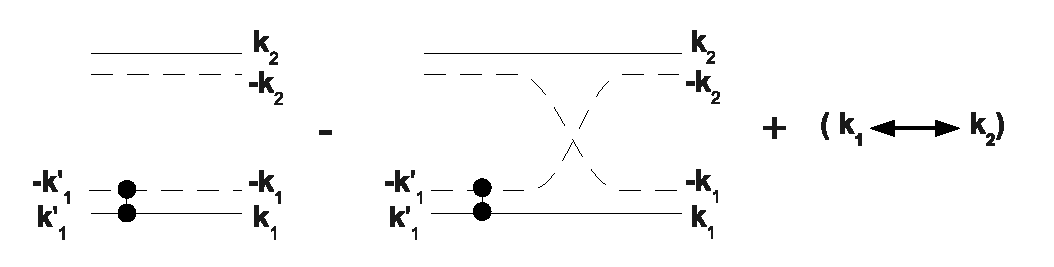
\includegraphics[width=0.45\textwidth]{twoPair.eps}
\caption{Shiva diagram for the interaction part $\left|v_{\mathbf{k} _1\mathbf{k} _2}\right>$ of the Hamiltonian $H$ acting on two free pairs, as given in Eq.(27)}
\label{fig:twoP}
\end{figure}


To go further, we subtract $E _2\beta^{\dagger}_{\mathbf{k}
_1}\beta^{\dagger}_{\mathbf{k} _2}\left|F_0\right>  $ to the two sides of Eq.%
\eqref{eq:SchTwo}, with $E _2$ yet undefined. We split $E _2$ as $R_1+R_2$ and we multiply
the resulting equation by $w_{\mathbf{k} _1}w_{\mathbf{k} _2}/\left(2%
\epsilon_{\mathbf{k} _1}-R_1\right) \left(2\epsilon_{\mathbf{k}
_2}-R_2\right) $. This yields


\begin{multline}  \label{eq:SchTwo2}
(H-E _2)B^{\dagger}_{\mathbf{k} _1}(R_1)B^{\dagger}_{\mathbf{k}
_2}(R_2)\left|F_0\right>   = \\
\left\{B^{\dagger}_{\mathbf{k} _1}(R_1)\left(w_{\mathbf{k}
_2}\beta^{\dagger}_{\mathbf{k} _2}-\frac{Vw_{\mathbf{k} _2}^2}{2\epsilon_{%
\mathbf{k} _2}-R_2}\beta^{\dagger}\right)+(1\leftrightarrow2)\right\}
\left|F_0\right>  \\
+2V\delta_{{\mathbf{k} _2}{\mathbf{k} _1}}\frac{w^3_{{\mathbf{k} _1}}\beta^\dagger_{{\mathbf{k} _1}}}{\left(2%
\epsilon_{\mathbf{k} _1}-R_1\right) \left(2\epsilon_{\mathbf{k}
_1}-R_2\right)}\beta^\dagger\left|F_0\right>  
\end{multline}
the last term coming from the exchange interaction part $\left|\omega_{\mathbf{k} _1\mathbf{k} _2}\right>$
To go further, we split $\left(2\epsilon_{\mathbf{k} _1}-R_1\right)
^{-1}\left(2\epsilon_{\mathbf{k} _1}-R_2\right) ^{-1}$ as $\left[%
\left(2\epsilon_{\mathbf{k} _1}-R_1\right) ^{-1}-\left(2\epsilon_{\mathbf{k}
_1}-R_2\right) ^{-1}\right] /\left(R_1-R_2\right) $ provided that $R_1\neq{}%
R_2$, a condition that we can always enforce since the unique requirement is to have $R_1+R_2=E_2$. This allows us to write the last term of \eqref{eq:SchTwo2} as $\delta_{{\mathbf{k} _2}{\mathbf{k} _1}}\frac{2V}{R_1-R_2}[B^{\dagger}_{\mathbf{k} _1}(R_1)-B^{\dagger}_{\mathbf{k} _1}(R_2)]\beta^\dagger\left|F_0\right>  $ provided that $w^2_{{\mathbf{k} }}=w_{{\mathbf{k} }}$. By taking sums over $\mathbf{k} _1$ and $\mathbf{k} _2$, Eq. %
\eqref{eq:SchTwo2} then gives 
\begin{multline}  \label{eq:SchTwo3}
(H-E_2)B^{\dagger}(R_1)B^{\dagger}(R_2)\left|F_0\right>   = \\
\left\{B^{\dagger}(R_1)\left(1-V\sum\frac{w_{\mathbf{k} }^2}{2\epsilon_{%
\mathbf{k} }-R_2}+\frac{2V}{R_1-R_2}\right) +(1\leftrightarrow2)\right\}  \\
\beta^{\dagger}\left|F_0\right>  
\end{multline}


The above equation readily shows that $B^{\dagger}(R_1)B^{\dagger}(R_2)%
\left|F_0\right>  $ is the two-pair eigenstate of the hamiltonian $H$ with the energy $%
E _2=R_1+R_2$ provided that $\left(R_1,R_2\right) $ fulfill two
equations, known as Richardson's equations for two pairs 
\begin{equation}
1=V\sum\frac{w_{\mathbf{k} }^2}{2\epsilon_{\mathbf{k} }-R_1}+\frac{2V}{R_1-R_2}%
=(1\leftrightarrow2)
\end{equation}

\subsection{Three pairs}

We now turn to three pairs in order to see how these equations develop for an
increasing number of pairs. We start with 
\begin{eqnarray}  \label{eq:SchThree}
&&H\beta^{\dagger}_{\mathbf{k} _1}\beta^{\dagger}_{\mathbf{k}
_2}\beta^{\dagger}_{\mathbf{k} _3}\left|F_0\right>  \hspace{5cm}
\nonumber\\
&=&\left\{\left[H,\beta^{\dagger}_{\mathbf{k} _1}\right]  \beta^{\dagger}_{%
\mathbf{k} _2}\beta^{\dagger}_{\mathbf{k} _3}+\beta^{\dagger}_{\mathbf{k} _1}%
\left[H,\beta^{\dagger}_{\mathbf{k} _2}\right]  \beta^{\dagger}_{\mathbf{k}
_3}\right.
\nonumber\\ &&\left.
+\beta^{\dagger}_{\mathbf{k} _1}\beta^{\dagger}_{\mathbf{k} _2}\left[%
H,\beta^{\dagger}_{\mathbf{k} _3}\right]  \right\}
\left|F_0\right> 
\end{eqnarray}%
 Eqs.(\ref{eq:betaH},\ref{eq:vbeta})  allow us to split the above equation into a kinetic part and an interaction part
\begin{equation}  \label{eq:SchThree2}
\begin{split}
H\beta^{\dagger}_{\mathbf{k} _1}\beta^{\dagger}_{\mathbf{k}
_2}\beta^{\dagger}_{\mathbf{k} _3}\left|F_0\right>   &=\left(2\epsilon_{%
\mathbf{k} _1}+2\epsilon_{\mathbf{k} _2}+2\epsilon_{\mathbf{k} _3}\right)
\beta^{\dagger}_{\mathbf{k} _1}\beta^{\dagger}_{\mathbf{k}
_2}\beta^{\dagger}_{\mathbf{k} _3}\left|F_0\right>   \\
&+\left|v_{\mathbf{k} _1\mathbf{k} _2\mathbf{k} _3}\right> 
\end{split}%
\end{equation}
The interaction part resulting from the BCS potential reads as 
\begin{equation}  \label{eq:vThree}
\begin{split}
\left|v_{\mathbf{k} _1\mathbf{k} _2\mathbf{k} _3}\right> =
\left(\gamma^{\dagger}_{\mathbf{k} _1}\beta^{\dagger}_{\mathbf{k}
_2}\beta^{\dagger}_{\mathbf{k} _3}+\gamma^{\dagger}_{\mathbf{k}
_2}\beta^{\dagger}_{\mathbf{k} _3}\beta^{\dagger}_{\mathbf{k}
_1}+\gamma^{\dagger}_{\mathbf{k} _3}\beta^{\dagger}_{\mathbf{k}
_1}\beta^{\dagger}_{\mathbf{k} _2}\right) \left|F_0\right>   \\
+\left(V^{\dagger}_{\mathbf{k} _1}\beta^{\dagger}_{\mathbf{k}
_2}\beta^{\dagger}_{\mathbf{k} _3}+\beta^{\dagger}_{\mathbf{k}
_1}V^{\dagger}_{\mathbf{k} _2}\beta^{\dagger}_{\mathbf{k} _3}+\beta^{%
\dagger}_{\mathbf{k} _1}\beta^{\dagger}_{\mathbf{k} _2}V^{\dagger}_{\mathbf{k%
} _3}\right) \left|F_0\right>  
\end{split}%
\end{equation}
Let us concentrate on the second part of $\left|v_{\mathbf{k} _1\mathbf{k} _2\mathbf{k} _3}\right> $. Its last term gives zero since $V^{\dagger}_\vk\left|F_0\right>  =0$. Using
Eq. \eqref{eq:vBeta}, the first two terms  can be
rewritten in a more symmetrical form as 
\begin{equation}  \label{eq:vThree2}
\begin{split}
&\left\{\left[V^{\dagger}_{\mathbf{k} _1},\beta^{\dagger}_{\mathbf{k} _2}%
\right]  \beta^{\dagger}_{\mathbf{k} _3}+\beta^{\dagger}_{\mathbf{k} _2}%
\left[V^{\dagger}_{\mathbf{k} _1},\beta^{\dagger}_{\mathbf{k} _3}\right] 
+\beta^{\dagger}_{\mathbf{k} _1}\left[V^{\dagger}_{\mathbf{k}
_2},\beta^{\dagger}_{\mathbf{k} _3}\right]  \right\} \left|F_0\right>   \\
=&\sum_{\vk^{\prime}_1\mathbf{k} ^{\prime}_2}\beta^{\dagger}_{\mathbf{k}
^{\prime}_1}\beta^{\dagger}_{\mathbf{k} ^{\prime}_2} \\
&\left\{\chi\left(\begin{smallmatrix}\vk'_2&\vk_2\\\vk'_1&\vk_1%
\end{smallmatrix}\right)  \beta^{\dagger}_{\mathbf{k} _3}+\chi\left(%
\begin{smallmatrix}\vk'_2&\vk_3\\\vk'_1&\vk_2\end{smallmatrix}\right) 
\beta^{\dagger}_{\mathbf{k} _1}+\chi\left(\begin{smallmatrix}\vk'_2&\vk_1\
\\\vk'_1&\vk_3\end{smallmatrix}\right)  \beta^{\dagger}_{\mathbf{k}
_2}\right\} \left|F_0\right>  
\end{split}%
\end{equation}

This leads us to represent the vector $\left|v_{\mathbf{k} _1\mathbf{k} _2%
\mathbf{k} _3}\right> $ by the diagram of Fig.\ref{fig:threeP}. It contains interactions inside a single pair, two pairs
staying unchanged. It also contains processes in which the pair suffering the potential exchange one fermion with a
second pair, the third pair staying unchanged. 
\begin{figure}[htb]
   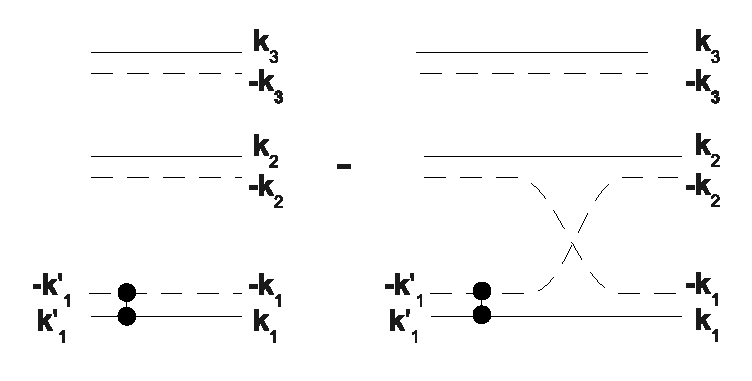
\includegraphics[width=0.4\textwidth]{threePair.eps}
\caption{Shiva diagram for the interaction part $\left|v_{\mathbf{k} _1\mathbf{k} _2%
\mathbf{k} _3}\right> $ of the Hamiltonian $H$ acting on three pairs }\label{fig:threeP}
 
\begin{flushleft}
 \normalsize	As given in Eqs. (\ref{eq:vThree},\ref{eq:vThree2}). $\left|v_{\mathbf{k} _1\mathbf{k} _2%
\mathbf{k} _3}\right> $ also contains two  contributions similar to the one
visualized in this figure, obtained by circular permutation.
\end{flushleft}
\end{figure}

Using Eq. \eqref{eq:interactSc} for the interaction scattering, the RHS of the above equation reduces to 

\begin{align*}
  &-2(\delta_{\mathbf{k} _1\mathbf{k} _2}\gamma^{\dagger}_{\mathbf{k} _1}\beta^{\dagger}_{\mathbf{k} _1}\beta^{\dagger}_{\mathbf{k} _3}+ \text{2 perm.})\left|F_0\right>\\
&= 2V(\delta_{\mathbf{k} _1\mathbf{k} _2}w_{\mathbf{k} _1}\beta^{\dagger}_{\mathbf{k} _1}\beta^{\dagger}_{\mathbf{k} _3}+ \text{2 perm.})\beta^{\dagger}\left|F_0\right>
\end{align*}




If we now come back to Eq.\eqref{eq:SchThree2}, subtract $E
_3\beta^{\dagger}_{\mathbf{k} _1}\beta^{\dagger}_{\mathbf{k}
_2}\beta^{\dagger}_{\mathbf{k} _3}\left|F_0\right>  $ to both sides, with $%
E _3$ written as $R_1+R_2+R_3$, and multiply the resulting equation
by $w_{\mathbf{k} _1}w_{\mathbf{k} _2}w_{\mathbf{k} _3}/\left(2\epsilon_{%
\mathbf{k} _1}-R_1\right) \left(2\epsilon_{\mathbf{k} _2}-R_2\right)
\left(2\epsilon_{\mathbf{k} _3}-R_3\right) $, we end with

\begin{eqnarray}  \label{eq:SchThree3}
&&(H-E _3)B^{\dagger}_{\mathbf{k} _1}(R_1)B^{\dagger}_{\mathbf{k}
_2}(R_2)B^{\dagger}_{\mathbf{k} _3}(R_3)\left|F_0\right>  \hspace{3cm}\nonumber\\
&=& \Bigl\{B^{\dagger}_{\mathbf{k} _1}(R_1)B^{\dagger}_{\mathbf{k}
_2}(R_2)\bigl(w_{\mathbf{k} _3}\beta^{\dagger}_{\mathbf{k} _3}-\frac{Vw_{%
\mathbf{k} _3}^2}{2\epsilon_{\mathbf{k} _2}-R_3}\beta^{\dagger}\bigr) \hspace{1cm}\nonumber\\
&&+\text{2 perm.} \Bigr\}\left|F_0\right> \hspace{1cm}\nonumber\\
&&+2V\Bigl\{B^{\dagger}_{\mathbf{k} _3}(R_3)\frac{\delta_{\mathbf{k} _1\mathbf{%
k} _2}w^3_{\mathbf{k} _1}}{\left(2\epsilon_{\mathbf{k} _1}-R_1\right)
\left(2\epsilon_{\mathbf{k} _1}-R_2\right) }\beta^{\dagger}_{\mathbf{k} _1}\hspace{1cm}\nonumber\\
&&\qquad+\text{2 perm.}\Bigr\} 
\beta^{\dagger}\left|F_0\right> \hspace{1cm} 
\end{eqnarray}
To go further, we again split $\left(2\epsilon_{\mathbf{k} _1}-R_1\right)
^{-1}\left(2\epsilon_{\mathbf{k} _1}-R_2\right) ^{-1}$ as $\left[%
\left(2\epsilon_{\mathbf{k} _1}-R_1\right) ^{-1}-\left(2\epsilon_{\mathbf{k}
_1}-R_2\right) ^{-1}\right] /\left(R_1-R_2\right) $ provided that $R_1\neq{}%
R_2$ and do the same for the two other products. By summing over $%
\left(\mathbf{k} _1,\mathbf{k} _2,\mathbf{k} _3\right) $, we end with

\begin{multline}  \label{eq:SchThree4}
(H-E _3)B^{\dagger}(R_1)B^{\dagger}(R_2)B^{\dagger}(R_3)\left|F_0%
\right>  = \\
\{B^{\dagger}(R_2)B^{\dagger}(R_3) \\
\left(1-V\sum\frac{w_{\mathbf{k} _1}^2}{2\epsilon_{\mathbf{k} _1}-R_1}-\frac{2V%
}{R_1-R_2}+\frac{2V}{R_3-R_1}\right)  \\
+\text{2 perm.}\}\beta^{\dagger}\left|F_0\right>  
\end{multline}

This leads us to  conclude that the three-pair state $%
B^{\dagger}(R_1)B^{\dagger}(R_2)B^{\dagger}(R_3)\left|F_0\right>  $ is
eigenstate of the hamiltonian $H$ with the energy $E _3=R_1+R_2+R_3$,
provided that $\left(R_1,R_2, R_3\right) $ fulfill the three equations, 
\begin{equation}
\begin{split}
1&=V\sum\frac{w_{\mathbf{k} }^2}{2\epsilon_{\mathbf{k} }-R_1}+\frac{2V}{R_1-R_2%
}+\frac{2V}{R_1-R_3} \\
1&=V\sum\frac{w_{\mathbf{k} }^2}{2\epsilon_{\mathbf{k} }-R_2}+\frac{2V}{R_2-R_3%
}+\frac{2V}{R_2-R_1} \\
1&=V\sum\frac{w_{\mathbf{k} }^2}{2\epsilon_{\mathbf{k} }-R_3}+\frac{2V}{R_3-R_1%
}+\frac{2V}{R_3-R_2}
\end{split}%
\end{equation}

\subsection{N pairs}

The above commutation technique can be easily extended to N pairs. As nicely
visualized by the diagrams of Figs.\ref{fig:twoP} and \ref{fig:threeP}, the
effect of the BCS potential on these N pairs splits into two sets of processes:
In one set, one pair is affected by the (1x1) scattering while the other $N-1
$ pairs stay unchanged. In the other set, this pair in addition has, before the interaction, a fermion
exchange with another pair, the remaining $N-2$
pairs staying unchanged. This understanding readily shows that an increase of pair number above two, does not really change the structure of the equations
since $N-2$ pairs stay unchanged, the pair which exchanges its fermions with the
pair suffering the interaction being just one among $(N-1)$ pairs.

Although the equations become more and more cumbersome to be explicitly
written, the procedure is rather straightforward once we have understood
that either $(N-1)$ or $(N-2)$ pairs stay unaffected in the interaction process. The
general form of the $N$-pair eigenstate ultimately appears as 
\begin{equation}  \label{eq:SchThreeN}
(H-E _N)B^{\dagger}(R_1)\cdots{}B^{\dagger}(R_N)\left|F_0\right>  =0
\end{equation}
with $E _N=R_1+\cdots+R_N$, these $R_N$'s being solutions of $N$ coupled
equations 
\begin{equation}
1=V\sum\frac{w_{\mathbf{k} }^2}{2\epsilon_{\mathbf{k} }-R_i}+\sum_{j\neq{i}}%
\frac{2V}{R_i-R_j}\quad\qquad \text{for}\; i=\left(1,...,N\right) 
\end{equation}

\subsection{Physical understanding}

This  derivation of the Richardson's equations has the main advantage to
possibly trace back the parts in these equations which are directly linked
to the Pauli exclusion principle between fermion pairs through electron exchanges. 

From a mathematical point of view, the link is rather obvious: In the
absence of terms in $V/(R_i-R_j)$, the $N$ equations for $R_i$ reduced to
the same equation \eqref{eq:SchOne}, so that the result would be $R^{(0)}_i=%
E _1$ for all $i$: The fact that the energy of $N$ pairs differs
from $N$ times the single pair energy $E_1$ thus comes from the set of $(R_i-R_j)$'s
different from zero.

Physically, the fact that $E _N$ differs from $NE _1$
comes from interactions between Cooper pairs. Due to the (1x1) form of the BCS
potential within the pair subspace, interaction between pairs can only be mediated by fermion
exchanges as clear from Fig. (\ref{fig:chi}). 
Interactions between pairs thus
are solely the result of the Pauli exclusion principle between pairs. This
Pauli blocking mathematically appears through the various $\delta_{\mathbf{p}
^{\prime}\mathbf{p} }$ factors in Pauli scatterings $\lambda(%
\begin{smallmatrix}\vp^\prime_2&\vp_2\\\vp_1'&\vp_1\end{smallmatrix})  $. It
is then easy to mathematically trace back the $(R_i-R_j)$ differences
 in the Richardson's equations to these $\delta$ factors.

In short, the Kronecker symbols in the Pauli scatterings of fermion pairs
come from states which are excluded by the Pauli exclusion principle. They induce the $2V/(R_i-R_j)$ terms
of the Richardson's equations which ultimately makes the energy of $N$ pairs different
from the energy of $N$ independent pairs.

Another important feature of the energy $E _N$ for $N$ pairs that
this  derivation explains in a rather clear way, is the fact that the
part of the $N$ pairs energy coming from interaction, namely $E _N-N%
E _1$ depends on $N$ as $N(N-1)$ only. Indeed, the diagram of Fig.\ref%
{fig:threeP} evidences the fact that, because the electron pairs of interest have one degree of freedom only, the (1x1) BCS potential
mixed with fermion exchanges between pairs, ends by producing effective scatterings which are (2x2) only.
In order to have terms in the energy in $N(N-1)(N-2)$, we need topologically connected
diagrams between 3 pairs. Since these do not exist, terms in $N(N-1)(N-2)$ and above, cannot exist in the energy of $N$ Cooper pairs, in agreement with Eq.(1) which also reads
\begin{equation}  \label{eq:en}
E _N=NE _1+N(N-1)\left(\frac{1}{\rho_0} +\frac{\epsilon_c}{%
N_\Omega}\right) 
\end{equation}

\section{Richardson's exact eigenstate versus BCS ansatz \label{sec:conn}}

A last very smart aspect of the Richardson's procedure is that it provides the 
\emph{exact} form of the eigenstate, namely 
\begin{equation}
B^{\dagger}(R_1)\cdots{}B^{\dagger}(R_N)\left|F_0\right>  
\end{equation}
with $B^{\dagger}(R)$ given by Eq.\eqref{eq:B}. The fact that by
construction all the $R_i$'s are different, strongly questions the standard
BCS ansatz for the condensed pair wave function which reduces to $\left(B^{\dagger}\right)
^N\left|F_0\right> $ when projected into the $N$-pair subspace: \emph{all} the pairs are condensed into the same state.

To discuss this problem on precise grounds, let us again consider two pairs. In
a previous work\cite{combescotBCS}, we have shown, that the ``Richardson's
energies'' in the case of two pairs read as $R_1=R+iR^{\prime}$ and $R_2=R-i{}R^{\prime}$ with $R$
and $R^{\prime}$ real. In the
large sample limit, i.e. for $1/\rho_0$ small,  the dominant terms of these real and imaginary parts are given by $R\approx\epsilon_c+1/%
\rho_0+\epsilon_c/\rho_0\Omega$ and $R^{\prime}\approx\sqrt{2\epsilon_c/\rho_0}$. By writting $B^{\dagger}(R_1)B^{\dagger}(R_2)$ as 
\begin{equation}
\left[B^{\dagger}(R)+B^{\dagger}(R_1)-B^{\dagger}(R)\right]\times \left[%
B^{\dagger}(R)+B^{\dagger}(R_2)-B^{\dagger}(R)\right] 
\end{equation}
we get from eq \eqref{eq:B} 
\begin{equation}
B^{\dagger}(R_1)B^{\dagger}(R_2)=\left[B^{\dagger}(R)\right]
^2+{R^{\prime}}^2\left\{C^{\dagger}_+C^{\dagger}_--2B^{\dagger}(R)D^{\dagger}%
\right\} 
\end{equation}
where we have set 
\begin{align}
C^{\dagger}_{\pm}&=\sum\frac{w_\vk}{\left(2\epsilon_\vk-R\right)
\left(2\epsilon_\vk-R\pm{}iR^{\prime}\right) }\beta^{\dagger}_\vk \\
D^{\dagger}&=\sum\frac{w_\vk}{\left(2\epsilon_\vk-R\right) \left[%
\left(2\epsilon_\vk-R\right) ^2+{}{R^{\prime}}^2\right] }\beta^{\dagger}_\vk
\end{align}

Eq.(45) shows that, in order to possibly replace $B^{\dagger}(R_1)B^{\dagger}(R_2)$ by $\left[B^{\dagger}(R)\right]
^2$ as in the BCS ansatz, we must neglect terms in $R'^2$, i.e., in $1/\rho_0$. We  actually find, at the lowest order in the inverse sample volume, i.e., in $1/\rho_0$, that
\begin{multline}  \label{eq:BB}
B^{\dagger}(R_1)B^{\dagger}(R_2)-\left[B^{\dagger}(\frac{E _2}{2})%
\right] ^2 \\
\approx \frac{2\epsilon_c}{\rho_0}\Bigl\{-2B^{\dagger}(E _1)\sum\frac{w_\vk}{\left(2\epsilon_\vk-%
E _1\right) ^3}\beta^{\dagger}_\vk\\ +\Bigl[\sum\frac{w_\vk}{%
\left(2\epsilon_\vk-E _1\right) ^2}\beta^{\dagger}_\vk\Bigr]
^2\Bigr\}  
\end{multline}
This shows that $B^{\dagger}(R_1)B^{\dagger}(R_2)$ can be
replaced by $\left(B^{\dagger}(E _2/2)\right) ^2$ provided that we
consider as negligeable the RHS of the above equation. This imposes to neglect terms in $1/\rho_0$. 
In this limit, $E_2$ reduces to $2E_1$, so that $B^{\dagger}(E _2/2)$  reduces to $%
B^{\dagger}(E _1)$: The
two-pair eigenstate would then just be the product of two non-interacting single pairs. If
instead, we want to include
change induced by Pauli blocking which brings the
energy per pair from $E _1$ to $E _2/2=E
_1+1/\rho_0+\epsilon_c/\rho_0\Omega$, we are led to replace $B^{\dagger}(R_1)B^{%
\dagger}(R_2)$ by the ``condensed two-pair state'' $\left(B^{\dagger}(E _2/2)\right) ^2$. This
however is inconsistent because we then keep in this two-pair
operator, contribution in $1/\rho_0$ which are as large as the ones we drop
by neglecting the RHS of Eq.\eqref{eq:BB}: In the case of two pairs, the replacement of
the exact eigenstate $B^{\dagger}(R_1)B^{\dagger}(R_2)\left|F_0\right>  $ by
a BCS-like condensed state $\left(B^{\dagger}(E _2/2)\right)
^2\left|F_0\right>  $ is fully inconsistent.

Actually, it is claimed that the validity of the BCS ansatz is restricted to the thermodynamical
limit, i.e., to $N$ very large. It is possible to show that in the dilute limit on the single pair scale, when $N$ increases, the $R_i$'s stay two by two complex conjugate while the $(R_i - R_j)$ differences get larger and larger. We thus hardly see how, 
starting from the exact form of the $N$-pair eigenstate $B^{\dagger}(R_1)\cdots{}B^{\dagger}(R_N)\left|F_0\right>  $ 
obtained by Richardson, we can possibly recover the BCS ansatz with the same 
creation operator for all  pairs when $N$ gets very large.

Let us stress that, 
to the best of our knowledge,  derivations of the validity of the BCS antsatz for the ground state of $N$ pairs
mainly concentrate on the energy it provides 
(see, e.g., \cite{Schrieffer} and references therein).
 We fully agree with the fact that the BCS
ansatz indeed gives the correct ground state energy for $N$ pairs because the energy obtained using this ansatz
is just the one we derived from the exact Richardson's procedure. However
agreement on the energy by no mean proves agreement on the wave function.
Many examples have been given in the past with wave functions very different
from the exact one, while giving the correct energy. Direct
experiments supporting the form of the ground state wave function seems to be even harder to achieve than the ones possibly checking the ground state energy given in Eq.(1). 
It thus seems to us necessary to carefully reconsider agreement 
with experiments in the light of the exact Richardson's wave function. 

The reduced potential used in standart BCS superconductivity has the great advantage to allow an analytical resolution of the $N$-body Schrodinger equation - which is not that frequent. It is however clear that this potential is highly simplified. A certain amount of corrections are needed to make this potential more realistic. These are going to destroy the possibility to derive the eigenstate analytically. Nevertherless, we wish to note that  the BCS ansatz for the wave function with all the pairs condensed into the \emph{same} state which is commonly considered as one of the essential features of superconductivity, has been worked out within this reduced BCS potential. To precisely compare this conventional ansatz with the exact solution of the model in the canonical ensemble is definitly of importance.

Finally, let us stress that the possible replacement of $B^{\dagger}(R_1)\cdots{}B^{\dagger}(R_N)%
\left|F_0\right>  $ by $\left(B^{\dagger}\right) ^N\left|F_0\right>  $ is
actually crucial to support the overall picture of
superconductivity we commonly have in mind, with all the pairs in the same state, ``as an army of
little soldiers, all walking similarly''. 
In a forthcoming paper, we are going to come back to the validity of the BCS 
ansatz in the thermodynamical limit, in the light of our recent analytical results on the Richardson's exact procedure.

\section{Conclusion}

We have rederived the Richardson's equations for $N$ Cooper pairs using a commutation technique for
opposite spin electron pairs with zero total momentum, similar to the one we have
developed for composite boson excitons. Almost half a century ago,
Richardson has succeeded to write down the \emph{exact form} of the eigenstate for an
arbitrary number $N$ of pairs. It reads in terms of $N$ energy-like
quantities $R_1,..., R_N$ which are solution of $N$ coupled non-linear
equations. This many-body problem is exactly solvable when the
interaction potential between $2N$ electrons with up and down spins is the BCS reduced potential provided that 
the interaction scattering is separable, $V_{\mathbf{k} ^{\prime}\mathbf{k} }=-V\,w_{\mathbf{k}
^{\prime}}w_{\mathbf{k} }$ with $w_{\mathbf{k}}^2=w_{\mathbf{k}}$.
Note that such a separable potential is also required to get
the energy of a single pair in a compact form, as obtained by Cooper.
Richardson managed to extend the exact one-Cooper pair solution to $N$ pairs by
decoupling them: This is done in a quite smart manner by splitting the $N$-pair energy $E_N$ as $R_1+\cdots+R_N$. 

The  derivation we here propose for the equations fulfilled by $R_1,\cdots,R_N$, allows us to trace back
the physical origin of the various terms in a transparent way. In
particular, this derivation clearly shows that $N$ pairs differ from $N$ independent
pairs, due to Pauli blocking only. This Pauli blocking
enforces the $R_i$ energy-like parameters of the Richardson's equations to be all different. 
As a direct consequence, the exact wave function for $N$ interacting pairs is 
definitely different from the BCS ansatz, although the $N$-pair energy this ansatz provides, is the same in the large sample limit. 

The diagrammatic
representation of this derivation nicely evidences that, because electron pairs
with zero total momentum have one degree of freedom only, they scatter within the $(1\times1)$ BCS potential in the pair subspace, through 
$(2\times2)$ scatterings only. This makes clearer
why the $N$-pair interaction energy that we have previously found, has interaction terms in $N(N-1)$ but not in $N(N-1)(N-2)
$ and so on... as commonly expected in $N$-body problems.

One of us (M.C.) wishes to thank the University of Illinois at
Urbana-Champaign, and Tony Leggett in particular, for enlightening discussions during a month invitation at
the Institute for Condensed Matter Physics where most of the present work has been
performed. We also wish to thank Walter Pogosov for his constructive comments on the manuscript.

\begin{thebibliography}{9}
\expandafter\ifx\csname natexlab\endcsname\relax\def\natexlab#1{#1}\fi
\expandafter\ifx\csname bibnamefont\endcsname\relax
  \def\bibnamefont#1{#1}\fi
\expandafter\ifx\csname bibfnamefont\endcsname\relax
  \def\bibfnamefont#1{#1}\fi
\expandafter\ifx\csname citenamefont\endcsname\relax
  \def\citenamefont#1{#1}\fi
\expandafter\ifx\csname url\endcsname\relax
  \def\url#1{\texttt{#1}}\fi
\expandafter\ifx\csname urlprefix\endcsname\relax\def\urlprefix{URL }\fi
\providecommand{\bibinfo}[2]{#2}
\providecommand{\eprint}[2][]{\url{#2}}
\providecommand \enquote [1]{``#1''}%
\providecommand \Eprint[0]{\href }%
\bibitem[{\citenamefont{Bardeen et~al.}(1957)\citenamefont{Bardeen, Cooper, and
  Schrieffer}}]{BCS}
\bibinfo{author}{\bibfnamefont{J.}~\bibnamefont{Bardeen}},
  \bibinfo{author}{\bibfnamefont{L.~N.} \bibnamefont{Cooper}},
  \bibnamefont{and} \bibinfo{author}{\bibfnamefont{J.~R.}
  \bibnamefont{Schrieffer}}, \bibinfo{journal}{Physical Review}
  \textbf{\bibinfo{volume}{106}}, \bibinfo{pages}{162} (\bibinfo{year}{1957}).

 \bibitem[{\citenamefont{Richardson}(1963)}]{Richardson1}
\bibinfo{author}{\bibfnamefont{R.~W.} \bibnamefont{Richardson}},
  \bibinfo{journal}{physics letters} \textbf{\bibinfo{volume}{3}},
  \bibinfo{pages}{277} (\bibinfo{year}{1963}).

\bibitem[{\citenamefont{Richardson and Sherman}(1964)}]{Richardson2}
\bibinfo{author}{\bibfnamefont{R.~W.} \bibnamefont{Richardson}}
  \bibnamefont{and} \bibinfo{author}{\bibfnamefont{N.}~\bibnamefont{Sherman}},
  \bibinfo{journal}{Nucl. Phys.} \textbf{\bibinfo{volume}{52}},
  \bibinfo{pages}{221} (\bibinfo{year}{1964}).


\bibitem[{\citenamefont{Dukelsky et~al.}(2004)\citenamefont{Dukelsky, Pittel, and Sierra}}]{Duk}
\bibinfo{author}{\bibfnamefont{J.}~\bibnamefont{Dukelsky}},
  \bibinfo{author}{\bibfnamefont{S.} \bibnamefont{Pittel}},
  \bibnamefont{and} \bibinfo{author}{\bibfnamefont{G.}
  \bibnamefont{Sierra}}, \bibinfo{journal}{Rev. Mod. Phys.}
  \textbf{\bibinfo{volume}{76}}, \bibinfo{pages}{643} (\bibinfo{year}{2004}).

\bibitem[{\citenamefont{Braun and von Delft}(1998)}]{delft}
\bibinfo{author}{\bibfnamefont{F.} \bibnamefont{Braun}}
  \bibnamefont{and} \bibinfo{author}{\bibfnamefont{J.}~\bibnamefont{von Delft}},
  \bibinfo{journal}{Phys. Rev. Lett.} \textbf{\bibinfo{volume}{81}},
  \bibinfo{pages}{4712} (\bibinfo{year}{1998}).


\bibitem[{\citenamefont{Richardson}(1965)}]{Richardson3}
\bibinfo{author}{\bibfnamefont{R.~W.} \bibnamefont{Richardson}},
  \bibinfo{journal}{J. Math. Phys.} \textbf{\bibinfo{volume}{18}},
  \bibinfo{pages}{1802} (\bibinfo{year}{1977}).
  
  \bibitem{paper1}
  W. Pogosov, M. Combescot, ArXiv. 0911.0849
  

\bibitem[{\citenamefont{Eagles}(1969)}]{Eagle}
\bibinfo{author}{\bibfnamefont{D.~M.} \bibnamefont{Eagles}},
  \bibinfo{journal}{Phys. Rev.} \textbf{\bibinfo{volume}{186}},
  \bibinfo{pages}{456} (\bibinfo{year}{1969}).

\bibitem[{\citenamefont{Leggett}(1980)}]{LeggettCrossover}
\bibinfo{author}{\bibfnamefont{A.~J.} \bibnamefont{Leggett}}, in
  \emph{\bibinfo{booktitle}{Proceedings of the XVIth Karpacz Winter School of
  Theoretical Physics, Karpacz, Poland}} (\bibinfo{publisher}{Springer-Verlag},
  \bibinfo{year}{1980}), pp. \bibinfo{pages}{13--27}.

\bibitem[{\citenamefont{Schrieffer}(1999)}]{Schrieffer}
\bibinfo{author}{\bibfnamefont{J.~R.} \bibnamefont{Schrieffer}},
  \emph{\bibinfo{title}{{Theory Of Superconductivity}}}
  (\bibinfo{publisher}{Perseus Books}, \bibinfo{year}{1999}),
  \bibinfo{edition}{revised edition} ed., ISBN \bibinfo{isbn}{0738201200}.

\bibitem[{\citenamefont{Combescot et~al.}(2008)\citenamefont{Combescot,
  Betbeder-Matibet, and Dubin}}]{CobosonPhysicsReports}
\bibinfo{author}{\bibfnamefont{M.}~\bibnamefont{Combescot}},
  \bibinfo{author}{\bibfnamefont{O.}~\bibnamefont{Betbeder-Matibet}},
  \bibnamefont{and} \bibinfo{author}{\bibfnamefont{F.}~\bibnamefont{Dubin}},
  \bibinfo{journal}{Physics Reports} \textbf{\bibinfo{volume}{463}},
  \bibinfo{pages}{215} (\bibinfo{year}{2008}).

  
  \bibitem{frenkel}  Wannier excitons have two degrees of freedom while Frenkel excitons, like Cooper pairs, have one only. This is why the Frenkel exciton many-body physics has similarities with the one of Cooper pairs (see  W. Pogosov, M. Combescot, Euro. Phys. J. B, Vol. 68, 161(2009) and Vol. 68, 183 (2009)).
  
  



\bibitem{combescotBCS}%
W. Pogosov, M. Combescot, M. Crouzeix ArXiv. 0911.1688
 
\end{thebibliography}
\end{document}
